
\begin{frame}{A Frame with two Columns}
  % 
  \begin{columns}
    %
    \begin{column}{.45\textwidth}
      \minipage[c][0.65\textheight][s]{\columnwidth}
      \vspace{0.05\textheight}
      
      On the left side text, figures on the right.

      \vfill

      \onslide<2->

      Start with basic figures, add more information later

      \vfill

      \onslide<3->

      Use \texttt{\textbackslash vfill} for the text column but not
      for figures.

      \vfill
      \onslide<4->
      \begin{tabular}{|p{0.9\textwidth}}
        Sometimes I change my mind and show a completely different
        figure on the right.
      \end{tabular}
   
      
      \endminipage      
    \end{column}
    %
    \begin{column}{.55\textwidth}
      \minipage[c][0.8\textheight][s]{\columnwidth}
      
      % Don't use \vfill in the image column!
      
      \onslide<1->

      \only<1-3>{
      \begin{figure}
        \centering
        \includegraphics<1>[width=\textwidth]{%
          img/figure1.png} %
        \includegraphics<2-3>[width=\textwidth]{%
          img/figure1_red.png} %
      \end{figure}}
      
      \only<3>{
      \begin{figure}
        \centering
        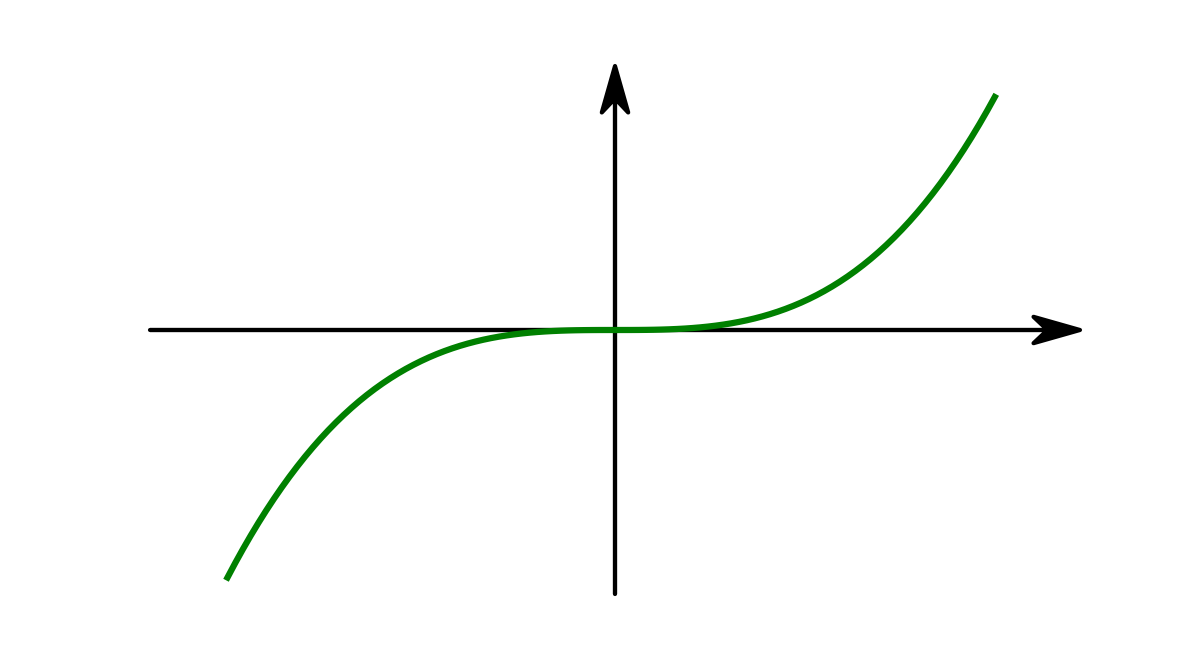
\includegraphics[width=\textwidth]{%
          img/figure2.png} %
      \end{figure}
      }

      \only<4>{

        \begin{figure}
          \vspace{1.2cm} % Here I don't know how else to vertically
                       % center the image
          \centering
          
\includegraphics[height=0.5\textheight]{%
            img/figure4.png} %
        \end{figure}
        \vfill
      } 

      
      \endminipage
    \end{column}
  \end{columns}

\end{frame}
